\documentclass[hidelinks,11pt]{book}

%These tell TeX which packages to use.
\usepackage{array,epsfig}
\usepackage{amsmath}
\usepackage{amsfonts}
\usepackage{amssymb}
\usepackage{amsxtra}
\usepackage{amsthm}
\usepackage{mathrsfs}
\usepackage{color}
\usepackage{graphicx} % adicionar figuras
\usepackage{float}

\usepackage{times}
\usepackage[T1]{fontenc}
\usepackage{setspace} % configurar espaçamento entre linhas
\usepackage{babel} %lingua portuguesa
\usepackage{microtype}
\usepackage{subcaption} % descrição de figuras
\usepackage[utf8]{inputenc}
\usepackage{blindtext}
\usepackage[round]{natbib}
\usepackage[a4paper, margin=2cm]{geometry} % margem
\usepackage{hyperref}

%Here I define some theorem styles and shortcut commands for symbols I use often
\theoremstyle{definition}
\newtheorem{defn}{Definition}
\newtheorem{thm}{Theorem}
\newtheorem{cor}{Corollary}
\newtheorem*{rmk}{Remark}
\newtheorem{lem}{Lemma}
\newtheorem*{joke}{Joke}
\newtheorem{ex}{Example}
\newtheorem*{soln}{Solution}
\newtheorem{prop}{Proposition}

\newcommand{\lra}{\longrightarrow}
\newcommand{\ra}{\rightarrow}
\newcommand{\surj}{\twoheadrightarrow}
\newcommand{\graph}{\mathrm{graph}}
\newcommand{\bb}[1]{\mathbb{#1}}
\newcommand{\Z}{\bb{Z}}
\newcommand{\Q}{\bb{Q}}
\newcommand{\R}{\bb{R}}
\newcommand{\C}{\bb{C}}
\newcommand{\N}{\bb{N}}
\newcommand{\M}{\mathbf{M}}
\newcommand{\m}{\mathbf{m}}
\newcommand{\MM}{\mathscr{M}}
\newcommand{\HH}{\mathscr{H}}
\newcommand{\Om}{\Omega}
\newcommand{\Ho}{\in\HH(\Om)}
\newcommand{\bd}{\partial}
\newcommand{\del}{\partial}
\newcommand{\bardel}{\overline\partial}
\newcommand{\textdf}[1]{\textbf{\textsf{#1}}\index{#1}}
\newcommand{\img}{\mathrm{img}}
\newcommand{\ip}[2]{\left\langle{#1},{#2}\right\rangle}
\newcommand{\inter}[1]{\mathrm{int}{#1}}
\newcommand{\exter}[1]{\mathrm{ext}{#1}}
\newcommand{\cl}[1]{\mathrm{cl}{#1}}
\newcommand{\ds}{\displaystyle}
\newcommand{\vol}{\mathrm{vol}}
\newcommand{\cnt}{\mathrm{ct}}
\newcommand{\osc}{\mathrm{osc}}
\newcommand{\LL}{\mathbf{L}}
\newcommand{\UU}{\mathbf{U}}
\newcommand{\support}{\mathrm{support}}
\newcommand{\AND}{\;\wedge\;}
\newcommand{\OR}{\;\vee\;}
\newcommand{\Oset}{\varnothing}
\newcommand{\st}{\ni}
\newcommand{\wh}{\widehat}

%Pagination stuff.
\setlength{\topmargin}{-.3 in}
\setlength{\oddsidemargin}{0in}
\setlength{\evensidemargin}{0in}
\setlength{\textheight}{9.in}
\setlength{\textwidth}{6.5in}
\pagestyle{empty}



\begin{document}
	
	
	\begin{center}
		{\Large Econometria I \hspace{0.5cm} Lista 1}\\
		Profa. Lorena Hakak\\
		Entrega: 03/10/2022
	\end{center}
	
	\vspace{0.2 cm}
	
	
	\subsection*{1.}

\subsubsection{(a)}

	\begin{center}
	\begin{tabular}{|c|c|c|c|c|}\hline
		K$\setminus$L & 0 & 1 & 2 & Prob(K)\\\hline
		-1 & 0,1 & 0,1 & 0,15 & \textcolor{red}{0,35}\\\hline
		0 & 0,15 & 0,1 & 0,1 & \textcolor{red}{0,35}\\\hline
		1 & 0,05 & 0,15& 0,1 & \textcolor{red}{0,3}\\\hline
		Prob(L) & \textcolor{red}{0,3} &\textcolor{red}{0,35}& \textcolor{red}{0,35} & 1\\\hline
	\end{tabular}
\end{center}


\begin{center}
	P(K = -1) = P(K=-1|L = 0) + P(K=-1|L = 1) + P(K=-1|L = 2)
\end{center}

\begin{center}
	P(K = -1) =0,1 + 0,1 + 0,15
\end{center}

\begin{center}
	P(K = -1) = 0,35
\end{center}

\begin{center}
	P(K = 0) = P(K=0|L = 0) + P(K=0|L = 1) + P(K=0|L = 2)
\end{center}

\begin{center}
	P(K = 0) = 0,15 + 0,1 + 0,1
\end{center}

\begin{center}
	P(K = 0) = 0,35
\end{center}

\begin{center}
	P(K = 1) = P(K=1|L = 0) + P(K=1|L = 1) + P(K=1|L = 2)
\end{center}

\begin{center}
	P(K = 1) = 0,05 + 0,15 + 0,1
\end{center}

\begin{center}
	P(K = 1) = 0,3
\end{center}


\begin{center}
	P(L = 0) = P(L=0|K = -1) + P(L = 0|K = 0) + P(L = 0|K = 1)
\end{center}

\begin{center}
	P(L = 0)  = 0,1 + 0,15 + 0,05
\end{center}

\begin{center}
	P(L = 0) = 0,3
\end{center}

\begin{center}
	P(L = 1) = P(L=1|K = -1) + P(L = 1|K = 0) + P(L = 1|K = 1)
\end{center}

\begin{center}
	P(L = 1)  = 0,1 + 0,1 + 0,15 
\end{center}

\begin{center}
	P(L = 1) = 0,35
\end{center}

\begin{center}
	P(L = 2) = P(L=2|K = -1) + P(L = 2|K = 0) + P(L = 2|K = 1)
\end{center}

\begin{center}
	P(L = 2)  =0,15 + 0,1 + 0,1
\end{center}

\begin{center}
	P(L = 2) = 0,35
\end{center}


\subsubsection{(b)}

\begin{displaymath}
	E(K) = \sum_{i = 1}^{3} k_i P[K = k_i]
\end{displaymath}

\begin{displaymath}
	E(K) = -1.(0,35) + 0.(0,35) + 1.(0,3)
\end{displaymath}

\begin{displaymath}
	E(K) = -0,05
\end{displaymath}

\begin{displaymath}
	E(L) = \sum_{i = 1}^{3} l_i P[L = l_i]
\end{displaymath}

\begin{displaymath}
	E(L) = 0. (0,3) + 1. (0,35) + 2. (0,35)
\end{displaymath}

\begin{displaymath}
	E(L) = 1,05
\end{displaymath}


\subsubsection{(c)}

	\begin{center}
	\begin{tabular}{|c|c|c|c|c|}\hline
		K & L & K.L & Prob(K,L) & K.L.Prob(K,L)\\\hline
		-1 & 0& 0 & 0,1 & 0\\\hline
		-1 & 1 & -1 & 0,1 &  -0,1\\\hline
		-1 & 2 & -2& 0,15 & -0,3\\\hline
		0 & 0& 0 & 0,15 & 0\\\hline
		0 & 1 & 0 & 0,1 &  0\\\hline
		0 & 2 & 0& 0,1 & 0\\\hline
		1 & 0& 0 & 0,05 & 0\\\hline
		1 & 1 & 1 & 0,15 &  0,15\\\hline
		1 & 2 & 2& 0,1 & 0,2\\\hline
	\end{tabular}
\end{center}

\begin{displaymath}
	E(KL) = \sum_{i = 1}^{3} k_i P[K = k_i].l_i P[L = l_i] = -0,05
\end{displaymath}


\begin{displaymath}
	COV(K,L) = E[KL] - E[K]E[L]
\end{displaymath}

\begin{displaymath}
	COV(K,L) = -0,05 - (-0,05)(1,05)
\end{displaymath}

\begin{displaymath}
	COV(K,L) = 0,0025
\end{displaymath}


\subsubsection{(d)}

K e L não são variáveis independentes, pois a covariância entre eles é diferente de zero:

\begin{displaymath}
	COV(K,L) \neq 0.
\end{displaymath}


\subsubsection{(e)}

Para $P(K|L = 1)$ nós temos:

\begin{displaymath}
P(K = -1|L = 1) = \frac{P(K = -1 \cap L = 1)}{P(L= 1)}= \frac{0,1}{0,35} = 0,28
\end{displaymath}

\begin{displaymath}
	P(K = 0|L = 1) = \frac{P(K = 0 \cap L = 1)}{P(L= 1)}= \frac{0,1}{0,35} = 0,28
\end{displaymath}

\begin{displaymath}
	P(K = 1|L = 1) = \frac{P(K = 1 \cap L = 1)}{P(L= 1)}= \frac{0,15}{0,35} = 0,43
\end{displaymath}

Portanto, $P(K|L = 1) = -1.(0,28) + 0.(0,28) + 1.(0,43) = 0,15$.\\

Para $P(L|K = 0)$ nós temos:

\begin{displaymath}
	P(L = 0|K = 0) = \frac{P(L = 0 \cap K = 0)}{P(K= 0)}= \frac{0,15}{0,35} = 0,43
\end{displaymath}


\begin{displaymath}
	P(L = 1|K = 0) = \frac{P(L = 1 \cap K = 0)}{P(K= 0)}= \frac{0,15}{0,35} = 0,28
\end{displaymath}

\begin{displaymath}
	P(L = 2|K = 0) = \frac{P(L = 2 \cap K = 0)}{P(K= 0)}= \frac{0,15}{0,35} = 0,28
\end{displaymath}

Portanto, $P(L|K = 0) = 0.(0,43) + 1.(0,28) + 2.(0,28) = 0,84$.

	\subsection*{2.}
\begin{figure}[H]
	\centering
	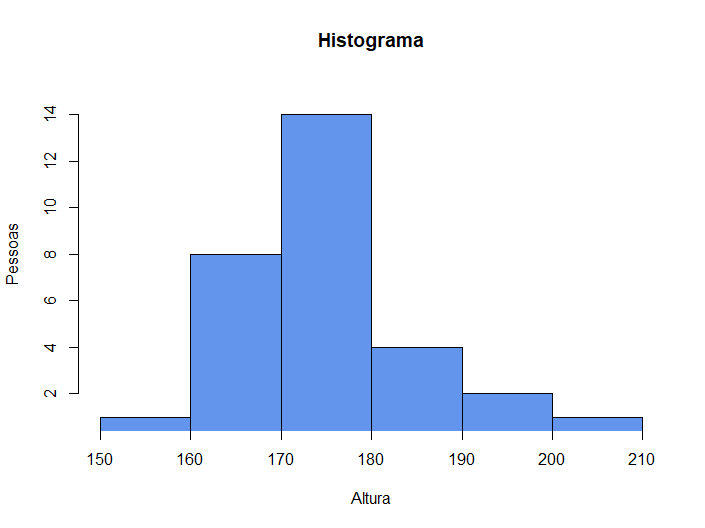
\includegraphics[width=0.7\linewidth]{Histograma}
	\caption*{}
\end{figure}





	\subsection*{3.}


Seja $X$ uma variável aleatória de média populacional  $\mu$ e média amostral $\frac{\sum_{i = 1}^{n} X_i}{n}=\overline{X}$. Logo:

\begin{displaymath}
	\overline{X} = \frac{\sum_{i = 1}^{n} X_i}{n}
\end{displaymath}

\begin{displaymath}
	E[\overline{X}] = E\Bigg[\frac{\sum_{i = 1}^{n} X_i}{n}\Bigg]
\end{displaymath}

\begin{displaymath}
	E[\overline{X}] = \frac{1}{n}E\Bigg[\sum_{i = 1}^{n} X_i\Bigg]
\end{displaymath}

\begin{displaymath}
	E[\overline{X}] = \frac{1}{n}\sum_{i = 1}^{n} E[X_i]
\end{displaymath}

\begin{displaymath}
	E[\overline{X}] = \frac{1}{n}\sum_{i = 1}^{n} \mu
\end{displaymath}

\begin{displaymath}
	E[\overline{X}] = \frac{1}{n}n.\mu
\end{displaymath}


\begin{displaymath}
	E[\overline{X}] = \mu.
\end{displaymath}



	
	\subsection*{4.}

\begin{displaymath}
	\frac{1}{n} \sum_{i = 1}^{n} (X_i - \overline{X})^2
\end{displaymath}

\begin{displaymath}
	\frac{1}{n} \sum_{i = 1}^{n} (X_i - \overline{X})(X_i - \overline{X})
\end{displaymath}

\begin{displaymath}
	\frac{1}{n} \sum_{i = 1}^{n} ({X_i}^2 - X_i\overline{X} -\overline{X} X_i + {\overline{X}}^2)
\end{displaymath}

\begin{displaymath}
	\frac{1}{n} \sum_{i = 1}^{n} ({X_i})^2 - \frac{1}{n} \sum_{i = 1}^{n}X_i\overline{X} - \frac{1}{n} \sum_{i = 1}^{n}X_i\overline{X} + \frac{1}{n} \sum_{i = 1}^{n}{\overline{X}}^2
\end{displaymath}

\vspace{2em}

Como $\frac{\sum_{i = 1}^{n} X_i}{n}=\overline{X}$ e $\frac{\sum_{i = 1}^{n}\overline{X}^2}{n}=\overline{X}^2$, então:


\begin{displaymath}
	\frac{1}{n} \sum_{i = 1}^{n} ({X_i})^2 - \overline{X}\overline{X} -\overline{X}\overline{X}  +  \overline{X}^2
\end{displaymath}

\begin{displaymath}
	\frac{1}{n} \sum_{i = 1}^{n} ({X_i})^2 - \overline{X}\overline{X} -\overline{X}\overline{X}  +  \overline{X}^2
\end{displaymath}

\begin{displaymath}
	\frac{1}{n} \sum_{i = 1}^{n} ({X_i})^2 -   \overline{X}^2
\end{displaymath}


Portanto, $\frac{1}{n} \sum_{i = 1}^{n} (X_i - \overline{X})^2$ = $\frac{1}{n} \sum_{i = 1}^{n} ({X_i})^2 -   \overline{X}^2$.



	\subsection*{5.}
	
\begin{displaymath}
	\frac{1}{n} \sum_{i = 1}^{n} (X_i - \overline{X}) (Y_i - \overline{Y})
\end{displaymath}

\begin{displaymath}
	\frac{1}{n} \sum_{i = 1}^{n} (X_iY_i -X_i\overline{Y} - Y_i\overline{X} + \overline{X}\overline{Y})
\end{displaymath}

\begin{displaymath}
	\frac{1}{n} \sum_{i = 1}^{n} X_iY_i - \frac{1}{n} \sum_{i = 1}^{n}X_i\overline{Y} - \frac{1}{n} \sum_{i = 1}^{n}Y_i\overline{X} + \frac{1}{n} \sum_{i = 1}^{n}\overline{X}\overline{Y}
\end{displaymath}

\vspace{2em}

Como $\frac{\sum_{i = 1}^{n} X_i}{n}=\overline{X}$, $\frac{\sum_{i = 1}^{n} Y_i}{n}=\overline{Y}$ e $\frac{\sum_{i = 1}^{n}\overline{X}\overline{Y}}{n}=\overline{X}\overline{Y}$ , então:

\vspace{2em}

\begin{displaymath}
	\frac{1}{n} \sum_{i = 1}^{n} X_iY_i - \overline{X}\overline{Y} - \overline{Y}\overline{X} + \overline{X}\overline{Y}
\end{displaymath}


\begin{displaymath}
	\frac{1}{n} \sum_{i = 1}^{n} X_iY_i - \overline{X}\overline{Y}
\end{displaymath}

\vspace{2em}

Portanto, $\frac{1}{n} \sum_{i = 1}^{n} (X_i - \overline{X}) (Y_i - \overline{Y})$ = $\frac{1}{n} \sum_{i = 1}^{n} X_iY_i - \overline{X}\overline{Y}$.

	\subsection*{6.}

Para entendermos o que é o erro quadrático médio, precisamos entender o conceito de erro. O erro amostral, nesse caso, seria o erro que cometemos ao estimar o parâmetro $\theta$ de uma variável qualquer pelo seu estimador $T$. Portanto, o erro quadrático médio seria:

\begin{displaymath}
	\textrm{EQM}(T; \theta) = E(e^2) = E(T - \theta)^2
\end{displaymath}

Fazendo as manipulações corretas\footnote{Explicação completa no livro \citet{m17} nas páginas 306 e 307.} chegamos na expressão:

\begin{displaymath}
	\textrm{EQM}(T; \theta) = Var(T) + V^2,
\end{displaymath}

onde $Var(T)$ é a variância do estimador $T$ e $V$ é o viés.\\

Vamos agora entender sua relação com a eficiência de um estimador. Para ser eficiente, o estimador tem que ser não viesado, e ter uma variância pequena. Portanto, como o EQM é a soma desses dois parâmetros, quanto menor o EQM, mais eficiente o estimador é.








	\subsection*{7.}


\subsubsection{(a)}

\begin{displaymath}
	\overline{X} = \frac{1}{n} \sum_{i = 1}^{n} x_i
\end{displaymath}

\begin{displaymath}
	\overline{X} = \frac{1.000 + 2.000 + 1.500 + 800 + 700}{5}
\end{displaymath}


\begin{displaymath}
	\overline{X} = R\$1.200,00
\end{displaymath}



\subsubsection{(b)}

\begin{displaymath}
	S^2 = \frac{1}{n-1} \sum_{i=1}^{n} (x_i - \overline{X})^2
\end{displaymath}

\begin{displaymath}
	S^2 = \frac{(1.000 - 1.200)^2 + (2.000 - 1.200)^2 + (1.500 - 1.200)^2 + (800 - 1.200)^2 + (700 - 1.200)^2}{5-1}
\end{displaymath}



\begin{displaymath}
	S^2 = \frac{40.000 + 640.000 + 90.000 + 160.000 + 250.000}{4}
\end{displaymath}

\begin{displaymath}
	S^2 = R\$295.000,00.
\end{displaymath}

\subsubsection{(c)}


\begin{displaymath}
	Var(\overline{X}_n) = Var\Bigg(\frac{x_1 + \dots + x_n}{n}\Bigg) = \frac{1}{n^2}Var(x_1 + \dots + x_n)
\end{displaymath}





Como a amostragem é aleatória, as variáveis $\{x_1 + \dots + x_n\}$ são independentes, de modo que:


\begin{displaymath}
	Var(\overline{X}_n) =  \frac{1}{n^2}Var(x_1 + \dots + x_n) = \frac{1}{n^2}[Var(x_1) + \dots + Var(x_n)]
\end{displaymath}

Sendo a variância constante em cada variável, nós temos:


\begin{displaymath}
	Var(\overline{X}_n) =  \frac{1}{n^2}[\sigma^2 + \dots + \sigma^2] = \frac{n\sigma^2}{n^2} = \frac{\sigma^2}{n}
\end{displaymath}

Portanto, $Var(\overline{X}_n) = \frac{\sigma^2}{n} = \frac{295000}{5} = R\$59.000,00.$






	\subsection*{8.}

$E(X) = 9$ e $\sigma = 2$. Logo, $Var(X) = \sigma^2 = 4$.

\begin{displaymath}
	E(W) = E \Bigg[ \frac{\sum_{i = 1}^{5} ix_i}{\sum_{i = 1}^{5} i} \Bigg]
\end{displaymath}

\begin{displaymath}
	E(W) = E\Bigg[\frac{1X_1 + 2X_2 + 3X_3 + 4X_4 + 5X_5}{1+ 2+ 3+ 4 + 5} \Bigg]
\end{displaymath}

\begin{displaymath}
	E(W) = \frac{1E(X_1) + E(2X_2) + 3E(X_3) + 4E(X_4) + 5E(X_5)}{15}
\end{displaymath}

\begin{displaymath}
	E(W) = \frac{(1 + 2+ 3+ 4 + 5)E(X)}{15}
\end{displaymath}

\begin{displaymath}
	E(W) = \frac{15.9}{15}
\end{displaymath}

\begin{displaymath}
	E(W) = 9.
\end{displaymath}

\begin{displaymath}
	Var(W) = Var\Bigg[ \frac{\sum_{i = 1}^{5} ix_i}{\sum_{i = 1}^{5} i} \Bigg]
\end{displaymath}

\begin{displaymath}
	Var(W) = \frac{Var[ \sum_{i = 1}^{5} ix_i]}{15^2} 
\end{displaymath}

\begin{displaymath}
	Var(W) = \frac{\sum_{i = 1}^{5}i^2Var[ x_i]}{15^2} 
\end{displaymath}

\begin{displaymath}
	Var(W) = \frac{\sum_{i = 1}^{5}i^24}{15^2} 
\end{displaymath}

\begin{displaymath}
	Var(W) = \frac{4(1 + 4 + 9 +16 + 25)}{255}
\end{displaymath}

\begin{displaymath}
	Var(W) = \frac{4(55)}{255}
\end{displaymath}

\begin{displaymath}
	Var(W) = 0,98.
\end{displaymath}



	\subsection*{9.}

	\subsubsection{(a)}
Dado que $\overline{X}= 110,3$, temos:
	\begin{center}
	\begin{tabular}{|c|c|c|}\hline
	$X_i$ & ($X_i$ - $\overline{X}$) &($X_i - \overline{X})^2$  \\\hline
	114  & 3,7 & 13,69 \\\hline
	112 & 1,7 & 2,89 \\\hline
	109 & -1,3 & 1,69 \\\hline
	123 & 12,7 & 161,29 \\\hline
	111 & 0,7 & 0,49 \\\hline
	99 & -11,3 & 127,69 \\\hline
	121 & 10,7 & 114,49 \\\hline
	113 & 2,7 & 7,29 \\\hline
	98 & -12,3 & 151,29 \\\hline
	103 & -7,3 & 53,29 \\\hline 
	\end{tabular}
\end{center}

$\sum_{1}^{10} (X_i - \overline{X})^2 = 634,1$. 


\begin{displaymath}
	\textrm{VAR}(X) = \frac{\sum_{1}^{10} (X_i - \overline{X})^2 }{n-1}
\end{displaymath}

\begin{displaymath}
	\textrm{VAR}(X) = \frac{634,1 }{9}
\end{displaymath}

\begin{displaymath}
	\textrm{VAR}(X) = 70,46.
\end{displaymath}

	\subsubsection{(b)}
Dado que $\overline{Y}= 76,4$, temos:
\begin{center}
	\begin{tabular}{|c|c|c|}\hline
		$Y_i$ & ($Y_i$ - $\overline{Y}$) &($Y_i - \overline{Y})^2$  \\\hline
		55  & -21,4 & 457,96 \\\hline
		61 & -15,4 & 237,16 \\\hline
		77 & 0,6 & 0,36 \\\hline
		66 & -10,4 & 108,16 \\\hline
		81 & 4,6 & 21,16 \\\hline
		95 & 18,6 & 345,96 \\\hline
		75 & -1,4 & 1,96 \\\hline
		77 & -1,4 & 1,96 \\\hline
		90 & 13,6 & 184,96 \\\hline
		87 & 10,6 & 112,36 \\\hline 
	\end{tabular}
\end{center}



$\sum_{1}^{10} (Y_i - \overline{Y})^2 = 1470,4$. 


\begin{displaymath}
	\textrm{VAR}(Y) = \frac{\sum_{1}^{10} (Y_i - \overline{Y})^2 }{n-1}
\end{displaymath}

\begin{displaymath}
	\textrm{VAR}(Y) = \frac{1470,4}{9}
\end{displaymath}

\begin{displaymath}
	\textrm{VAR}(Y) =163,38.
\end{displaymath}



\subsubsection{(c)}

\begin{center}
	\begin{tabular}{|c|c|c|}\hline
		($X_i$ - $\overline{X}$) & ($Y_i$ - $\overline{Y}$) &($X_i$ - $\overline{X}$)($Y_i$ - $\overline{Y}$)  \\\hline
		3,7  & -21,4 & -79,18 \\\hline
		1,7 & -15,4 & -26,18 \\\hline
		-1,3 & 0,6 & -0,78 \\\hline
		12,7 & -10,4 & -132,08 \\\hline
		0,7 & 4,6 & 3,22 \\\hline
		-11,3 & 18,6 & -210,18 \\\hline
		10,7 & -1,4 & -14,98 \\\hline
		2,7 & -1,4 & 1,62 \\\hline
		-12,3 & 13,6 & -167,28 \\\hline
		-7,3 & 10,6 & -77,38 \\\hline 
	\end{tabular}
\end{center}

$\sum_{1}^{10}  (X_i - \overline{X})(Y_i - \overline{Y}) = -703,2$



\begin{displaymath}
	\textrm{COVAR}(X,Y) = \frac{\sum_{1}^{10}  (X_i - \overline{X})(Y_i - \overline{Y}) }{n-1}
\end{displaymath}

\begin{displaymath}
	\textrm{COVAR}(X,Y) = \frac{-703,2 }{9}
\end{displaymath}

\begin{displaymath}
	\textrm{COVAR}(X,Y) =-78,13.
\end{displaymath}

\subsubsection{(d)}

Sendo VAR($X$) = $\sigma_x^2$ e  VAR($Y$) = $\sigma_y^2$, o desvio-padrão das variáveis são:

\begin{displaymath}
	\sigma_x = \sqrt{\sigma_x^2}
\end{displaymath}

\begin{displaymath}
	\sigma_x = \sqrt{70,46}
\end{displaymath}

\begin{displaymath}
	\sigma_x = 8,39.
\end{displaymath}

Para $Y$:

\begin{displaymath}
	\sigma_y = \sqrt{\sigma_y^2}
\end{displaymath}

\begin{displaymath}
	\sigma_y = \sqrt{163,38}
\end{displaymath}

\begin{displaymath}
	\sigma_x = 12,78.
\end{displaymath}


Com o desvio-padrão de cada variável calculado, podemos encontrar a correlação entre elas. Partindo da fórmula:


\begin{displaymath}
	\textrm{correl}(X,Y) =\frac{\textrm{COVAR}(X,Y)}{\sigma_x \sigma_y}
\end{displaymath}

\begin{displaymath}
	\textrm{correl}(X,Y) =\frac{-78,13}{(8,39).(12,78)}
\end{displaymath}

\begin{displaymath}
	\textrm{correl}(X,Y) = -0,73.
\end{displaymath}



	\subsection*{10.}


\begin{displaymath}
	P( 19.000 \leq X \leq 25.000) = P(19.000 - 20.000 \leq X - 20.000 \leq 25.000 - 20.000)
\end{displaymath}

\begin{displaymath}
	P( 19.000 \leq X \leq 25.000) = P\Bigg(\frac{19.000 - 20.000}{4.000} \leq \frac{X - 20.000}{4.000} \leq \frac{25.000 - 20.000}{4.000}\Bigg)
\end{displaymath}


\begin{displaymath}
	P( 19.000 \leq X \leq 25.000) = P[-0,25 \leq z \leq 1,25]
\end{displaymath}

\vspace{2em}

Sendo $P(-0,25) = P(0,25)$, então:

\vspace{2em}

\begin{displaymath}
	P( 19.000 \leq X \leq 25.000) = P[z \geq 0,25] + P(z \leq 1,25)
\end{displaymath}

\begin{displaymath}
	P( 19.000 \leq X \leq 25.000) = 0,0987 + 0,3944
\end{displaymath}

\begin{displaymath}
	P( 19.000 \leq X \leq 25.000) = 0,4931.
\end{displaymath}

A probabilidade do faturamento estar entre $R\$ 19.000,00$ e $R\$ 25.000,00$ é de 49,31\%.

	\subsection*{11.}

	\subsubsection{(a)}


		
Dado que $ n = 49$, $\overline{X} = 820,00$ e $\sigma_x = 140,00$, a variância da média seria:

\begin{displaymath}
	\sigma_{\overline{X}} = \frac{\sigma_x}{\sqrt{49}} = \frac{140}{7} = 20.
\end{displaymath}

Como a distribuição normal padrão é simétrica em relação à média zero, 80\% de confiança significa 40\% para cada lado. Assim, vem, que:

\begin{displaymath}
	z_{40\%} = 1,28
\end{displaymath}

\begin{displaymath}
	IC(\mu;80) = 820 \pm 1,28.20 = 820 \pm 25,60.
\end{displaymath}

	\subsubsection{(b)}

\begin{displaymath}
	z_{45\%} = 1,64
\end{displaymath}

\begin{displaymath}
	IC(\mu;90) = 820 \pm 1,64.20 = 820 \pm 32,80.
\end{displaymath}

	\subsubsection{(c)}

Ao aumentarmos o intervalo de confiança, aumenta-se consequentemente a margem de erro. Isso porque teremos que ter mais certeza que os eventos irão ocorrer naquele intervalo.


	\subsubsection{(d)}

Para satisfazer as condições de margem de erro no máximo 20 e confiança de 90\%, é necessário que:

\begin{displaymath}
	1,64.\frac{140}{\sqrt{n}} \leq 20
\end{displaymath}


\begin{displaymath}
	1,64.\frac{140}{20} \leq \sqrt{n}
\end{displaymath}

\begin{displaymath}
	11,48 \leq \sqrt{n}
\end{displaymath}

\begin{displaymath}
	131,79 \leq n.
\end{displaymath}

Para que o erro seja de no máximo 20 com confiança de 90\% é necessário no mínimo 132 observações.

\clearpage


\begin{figure}[H]
	\centering
	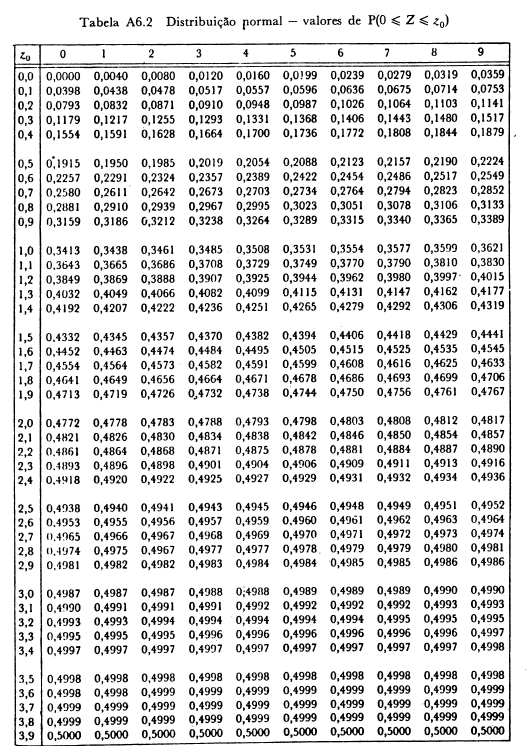
\includegraphics[width=0.7\linewidth]{tabela}
	\caption{}
	\label{fig:tabela}
\end{figure}






\bibliographystyle{apa}
\bibliography{reference}
	
	
\end{document}


